\chapter{Measuring Performance} \label{chap:perf}

% \tdo{Re-read this}
% \tdo{Maybe expand on the Accuracy and why it is bad}

% \begin{epiquote} 
%  \textit{When a measure becomes a target, it ceases to be a good measure.}
% \end{epiquote}    
% \begin{flushright} - \textit{Goodhart's Law}\end{flushright}\bigskip

 It is important to understand the benefits and downsides of using a specific measure when training a machine learning system. In this Appendix, a framework for theoretical rule analysis \cite{furnkranz2005roc} will be presented (Section \ref{chap:perf:background}). This framework will then be used to compare several common performance measures (Section \ref{chap:perf:measures}). Consideration will be made for the specific challenges presented by this work (i.e. the imbalance between the number of chronic and not chronic clients), however, this appendix will not be using data from the DI, and will instead focus on the theoretical use of the presented measures. 


\section{Background} \label{chap:perf:background}

% 35 if my counting is correct
There are over 30 measures for comparing binary classification systems in Foundations of Rule Learning \cite{furnkranz2012foundations}. However, each measure presents a specific trade-off between reinforcing true positives and penalizing false positives (or reinforcing true negatives and penalizing false negatives). Understanding this trade-off is of utmost importance when selecting a measure as it directly translates to the usefulness of the generated model.

This work is performed within the context, of housing operations where, due to budget and housing constraints, it is infeasible to house every client. In the standard classification context it is generally considered equal to increase the covered true positives or to decrease the covered false positives. However, in this context, adding additional covered clients can mean exceeding the capacity of a housing program. With this work, there will be a preference for decreasing the covered false positives when given the opportunity. Unfortunately, this trade-off is often unclear when looking at a measure definition, ideally, there would be a way to visualize this trade-off for each measure.

Receiver Operating Characteristic (ROC) \cite{Fawcett2006AnIT} analysis is a popular method of visualizing classifier performance. While the most common usage is the ROC curve, ROC analysis can take other forms. F{\"u}rnkranz and Flach \cite{furnkranz2005roc} demonstrate a method of using the ROC space to visualize the inherent true positive/false positive trade-off presented by different measures.

In this appendix, a modification of ROC space, called coverage space \cite{furnkranz2005roc}, will be used to visualize the differences between the measures. Coverage space only differs from ROC space in that it plots the number of true positives vs. false positives, rather than the true positive rate and false positives rate typically used in ROC space. 
In most cases, the plots will be almost identical between coverage space and ROC space, but coverage space tends to more accurately represent a measure by using the non-normalized values. This is particularly helpful when analyzing rules in the context of a skewed data set.

The rest of this appendix will adopt the notation used in Foundations of Rule Learning \cite{furnkranz2012foundations}. Within this appendix, these are purely theoretical values and not the result of having run any form of classifier. However, later appendix will adopt the same notation when presenting classification results.


\begin{align*}
	\mathcal{E} &= \text{Set of all examples (set of all clients)} \\
	\mathcal{P} &= \text{Set of positive examples} \\
	\mathcal{N} &= \text{Set of negative examples} \\
	P &= \text{Number of positive examples} = \hat P + \bar P = |\mathcal{P}| \\
	N &= \text{Number of negative examples} = \bar N + \hat N |\mathcal{P}| \\
	\hat P &= \text{Number of correct positive classifications (True positives)} \\
	\hat N &= \text{Number of incorrect positive classifications (False positives)} \\
	\bar P &= \text{Number of incorrect negative classifications (False negatives)} \\
	\bar N &= \text{Number of correct negative classifications (True negatives)} \\
\end{align*}


In this appendix only the set sizes will be used ($P, N, \hat P, \hat N, \bar P, \bar N$). Within figures, TP and FP will be used instead of $\hat P$ and $\hat N$ respectively.

Table \ref{tbl:perf:examples} presents two example classifications. These classifications are completely fabricated and are only represented by the confusion values. These examples will be used in the following section to compare the performance of different measures. These examples are created from a sample of 200 individual classifications. The Random example is an example of a randomized classifier, i.e. the classifier used predicts True 70\% of the time no matter what. The Good example is completely fabricated and demonstrates a pretty good classification. More examples will be introduced in the next section as needed.

\begin{table}[h]
	\centering

	\begin{tabular}{lrrrr}
	\toprule
	{} &    $\hat P$ & $\hat N$ & $\bar N$ & $\bar P$ \\
	\midrule
	Random & 70 & 70 & 30 & 30 \\
	Good   & 98 & 16 & 84 & 2  \\
	\bottomrule
	\end{tabular}

	\caption{Example classifications.}
	\label{tbl:perf:examples}
\end{table}


\section{Measures} \label{chap:perf:measures}

In this section, the three measures from association rule learning (Support, Confidence, and Lift) will be presented along with the Relative Linear Cost (RelLinCost) measure and the Accuracy measure.
The justification for selecting these measures is due to their popularity within the fields of association rule learning, classification rule learning, and machine/deep learning respectively.
The analysis taken in this section follows the one done by F{\"u}rnkranz and Flach, 2005 \cite{furnkranz2005roc} \cite{furnkranz2012foundations}, with a focus on the above rules.


First, a brief introduction into using coverage space as a tool for comparing measures. In typical usage of ROC space, the results of a single classification will be plotted ($\hat P$ and $\hat N$) as a point, and multiple classifications can be plotted by tweaking a threshold or a parameter in the classifier. When multiple classifications are plotted it will form a curve through the ROC space, called an ROC curve.

Points in the upper left corner of the plot $(0, P)$ (or lines that cross this point) are ideal because the corner represents a perfect prediction. Points in the bottom right are also good because the model can be inverted to obtain perfect predictions. Any point lying along the line $\hat P = \hat N$ is considered to be equivalent to a random guess because the probability of a true positive is equal to the probability of a false positive ($\text{P}(\hat P) = \text{P}(\hat N)$). A good measure will assign any point along this line a low score, and assign the maximum score to the point $(0, P)$. In the case where $P = N$, this line has a slope of 1, however, when used in the presence of class imbalance ($P \neq N$), the slope will be $P/N$. Because of the slope change, the line will always stretch from the bottom left corner to the top right corner of the coverage space. 

F{\"u}rnkranz and Flach's use of the coverage space does not depend on having classification results. They instead produce a 3D plot of a measure evaluation over the entire range of $\hat P$ and $\hat N$. This measure evaluation is a surface in 3D space. The gradient of this plot gives insight into the trade-off between true positives and false negatives. This 3D plot is represented in two dimensions using just the isometrics. An isometric is a line that represents all measures of the same value. Looking at a plot of isometrics is the same as looking at a 2D height map, the gradient can be observed as being perpendicular to the isometrics.
 
To demonstrate this the MinFP (Minimum False Positive) measure is introduced
$MinFP(\hat P, \hat N) = 1-\frac{\hat N}{N}$
. The MinFP measure is a simple measure that tracks how small the value of $\hat N$ is for a classifier. That is, a classifier with a low value of $\hat N$ will have a high MinFP score.

Figure \ref{fig:minfp} demonstrates the resulting isometric plot, which shows that the isometrics are equally spaced vertical lines. Any point along these vertical lines has the same MinFP value. The intuition that comes from looking at this plot is that MinFP does not properly account for true positives. This is rather obvious from the definition, and in the case of MinFP, the isometric plot is not very informative but stands as an example of the format.

This can be seen further by comparing the Good classification and an example classification that has the same MinFP score. It is clear from Figure \ref{fig:minfp} that the Match example is worse than the Good example, yet will still have the same MinFP score.

\begin{figure}[ht]
    \centering
    \figuretitle{Min FP}
    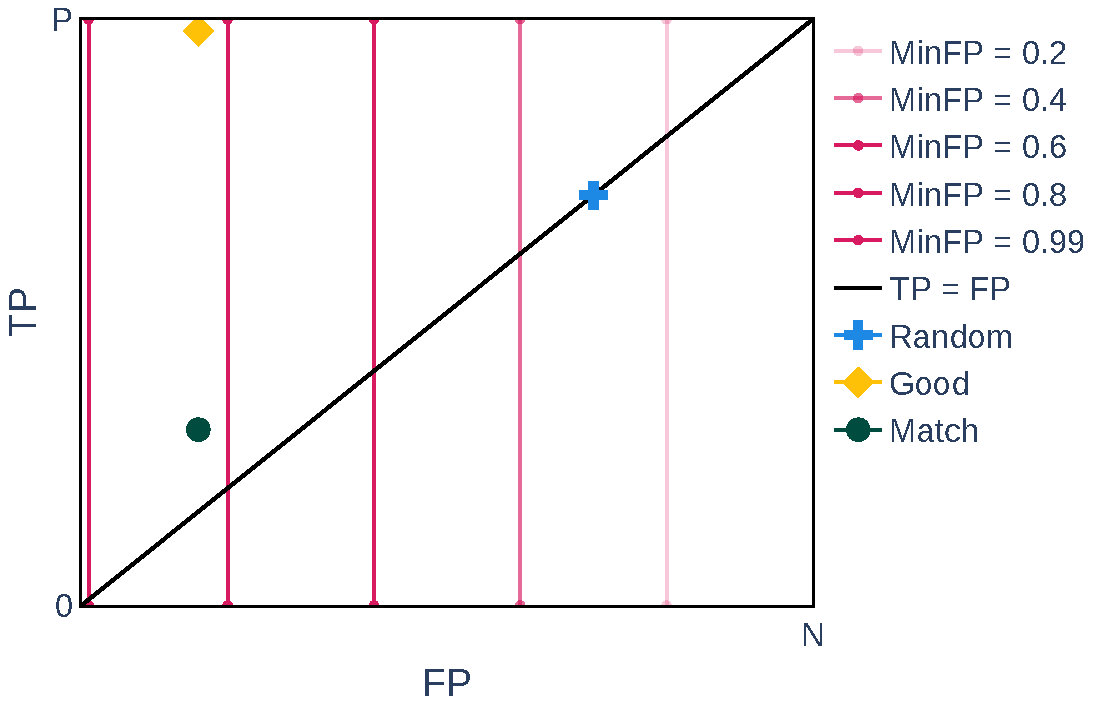
\includegraphics[width=0.7\textwidth]{Figures/MP-MinFP}
		\caption{Isometric plot for the MinFP measure.}
    \label{fig:minfp}
\end{figure}


\FloatBarrier
\subsection{Accuracy}

Accuracy is perhaps the most well-known measure, if only due to its familiar name. The reason for this popularity is clear when looking at the isometrics (Figure \ref{fig:accuracy}), which are parallel to the center line and evenly step towards the top left corner of the coverage space plot. This aligns exactly with the intuition one would develop from looking at the ROC/coverage space. The definition of Accuracy:
$Accuracy(\hat P, \hat N) = \frac{\hat P + \bar N}{P + N}$
demonstrates the reason for these isometrics, namely that Accuracy considers both true positives and true negatives in equal proportion, scaled by the total number of samples.

Intuitively, Accuracy is the proportion of correct classifications. An Accuracy of 1.0 (100\%) is thus the optimal metric, and a score of 0.5 (50\%) corresponds to a random guess. This is a good heuristic when $P \approx N$, however, it falls apart when $P$ and $N$ diverge. Figure \ref{fig:accuracy-bias} demonstrates such a case where $P = 0.2 N$, as can be seen, the isometrics skew towards the over-represented class and even relatively large changes in the minority class have little effect on the Accuracy score. This also corrupts the intuitive understanding of Accuracy as the $\hat P = 0.2 \hat N$ line is no longer aligned with an Accuracy score of 0.5. 

Figures \ref{fig:accuracy} and \ref{fig:accuracy-bias} use an additional example also called Match with values of 0.84, 0.02, 0.98, and 0.16 for $\hat P$, $\hat N$, $\bar N$, and $\bar P$ respectively. In the balanced class case $P=N$, the Random classifier has an Accuracy of 0.5, while the Good and Match classifiers have an Accuracy of 0.91. In the case with class imbalance ($P = 0.2 N$), the Random classifier now has an Accuracy of 0.7, the Good classifier has an Accuracy of 0.86, and the Match classifier has an Accuracy of 0.96.

This behaviour is undesirable for two reasons. The first is that the relative ordering of the Good and Match examples has changed when the underlying class distribution changed. This means that any classifier that uses Accuracy during the training phase will be extremely sensitive to the class distribution of the underlying data. For example, a classifier might be trained on a data set with a class distribution of X, and an Accuracy of 0.96. This classifier can then be employed on a new data set with class distribution Y, and an Accuracy of 0.8, even though the performance in terms of $\hat P$ and $\hat N$ might be identical. The second reason is that users of this system will not be able to build a proper intuition around what Accuracy means. Looking at the Random example, the Accuracy in the imbalanced case (0.7) appears good but still corresponds to a random guess.

 % Transparency is key in this work meaning that the lack of intuitive interpretation for Accuracy when working with the DI data ($P \approx 0.04 N$) makes it unsuitable for use.

\begin{figure}[ht]
    \centering
    \figuretitle{Accuracy}
    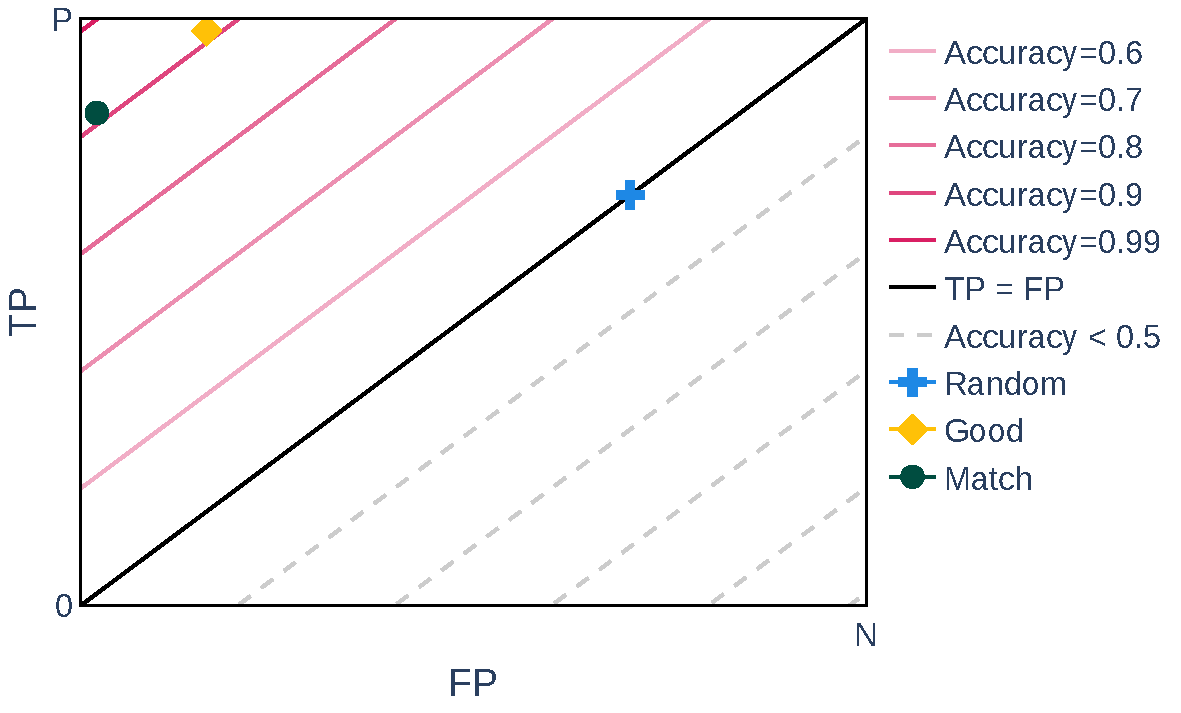
\includegraphics[width=0.7\textwidth]{Figures/MP-Accuracy}
		\caption{Isometric plot for the Accuracy measure.}
    \label{fig:accuracy}
\end{figure}
\begin{figure}[ht]
    \centering
    \figuretitle{Accuracy; P = 0.2 N}
    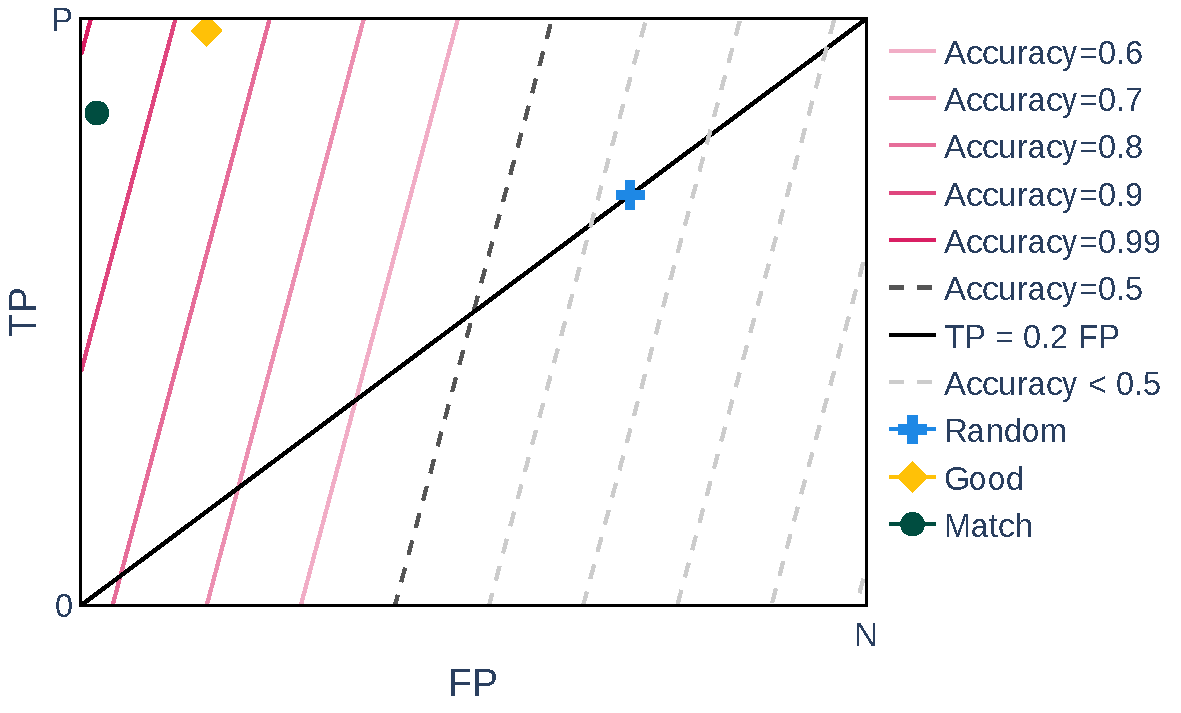
\includegraphics[width=0.7\textwidth]{Figures/MP-Accuracy-bias}
		\caption{Isometric plot for the Accuracy measure with a skewed class distribution.}
    \label{fig:accuracy-bias}
\end{figure}

\FloatBarrier
\subsection{Relative Linear Cost}

RelLinCost is a popular measure \cite{furnkranz2012foundations} within the field of classification rule learning. It is similar to Accuracy in that the isometrics perfectly sweep from the mid-line to the top-left corner (Figure \ref{fig:rellincost}). However, RelLinCost differs from Accuracy when working on an unbalanced data set. 
This is due to the configurable parameters $a$ and $b$ which can be seen in the definition of RelLinCost
$RelLinCost(\hat P, \hat N, a, b) = a  \frac{\hat P}{P} - b \frac{\hat N}{N}$
. This allows the system designer to configure a trade-off between true positives and false positives based on the specifics of the problem. A common use case is to have $a=1$ and $b=1$ which place equal importance on maximizing the true positive rate and minimizing the false positive rate. This presents a powerful tool in terms of designing a training system with configurable priorities.

RelLinCost can be seen as a generalization of Accuracy. Equation \ref{eq:rellincost-derive} demonstrates how the variables $a$ and $b$ can be configured to approximate Accuracy. This is only an approximation due to the dangling $\frac{N}{P+N}$, fortunately, this term will be constant and will not affect the relative ordering for model scores.

Because RelLinCost compares the rates rather than raw values, it will not suffer from the same issues as Accuracy when the underlying class distribution changes. Figure \ref{fig:rellincost-bias} demonstrates the case where $P = 0.2 N$. As can be seen in Figure \ref{fig:rellincost-bias} the isometrics of RelLinCost do not change when underlying class distribution changes (but can be adjusted using $a$ and $b$).

Additionally, the position of the three example points does not move when the class imbalance is introduced. This means that the intuition that users build up around what RelLinCost means will not change when the underlying class distribution changes. This makes RelLinCost an exceptionally robust measure.

\begin{equation} \label{eq:rellincost-derive}
    \begin{split}
    a = \frac{P}{P+N}; &\quad
    b = \frac{N}{P+N} \\
		RelLinCost(\hat P, \hat N, a, b) &= Accuracy(\hat P, \hat N) - \frac{N}{P+N}
    \end{split}
\end{equation}
\begin{figure}[ht]
    \centering
    \figuretitle{Relative Linear Cost}
    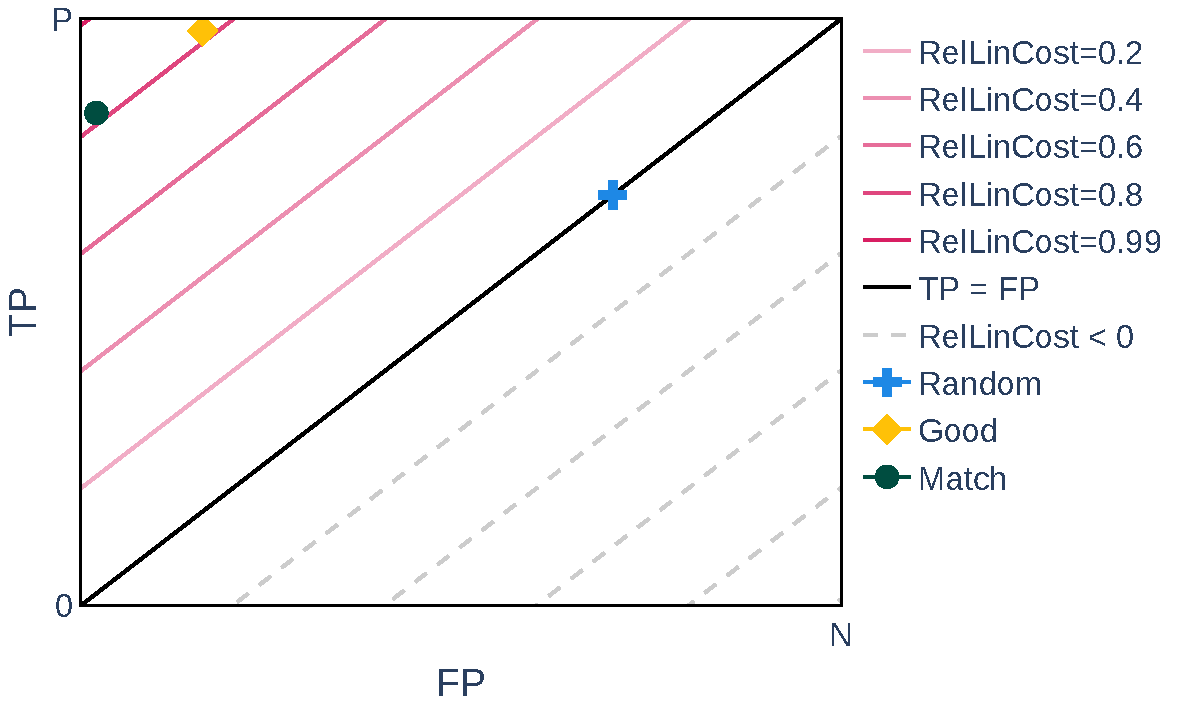
\includegraphics[width=0.7\textwidth]{Figures/MP-RelLinCost}
		\caption{Isometric plot for the RelLinCost measure.}
    \label{fig:rellincost}
\end{figure}
\begin{figure}[ht]
    \centering
    \figuretitle{Relative Linear Cost; P = 0.2 N}
    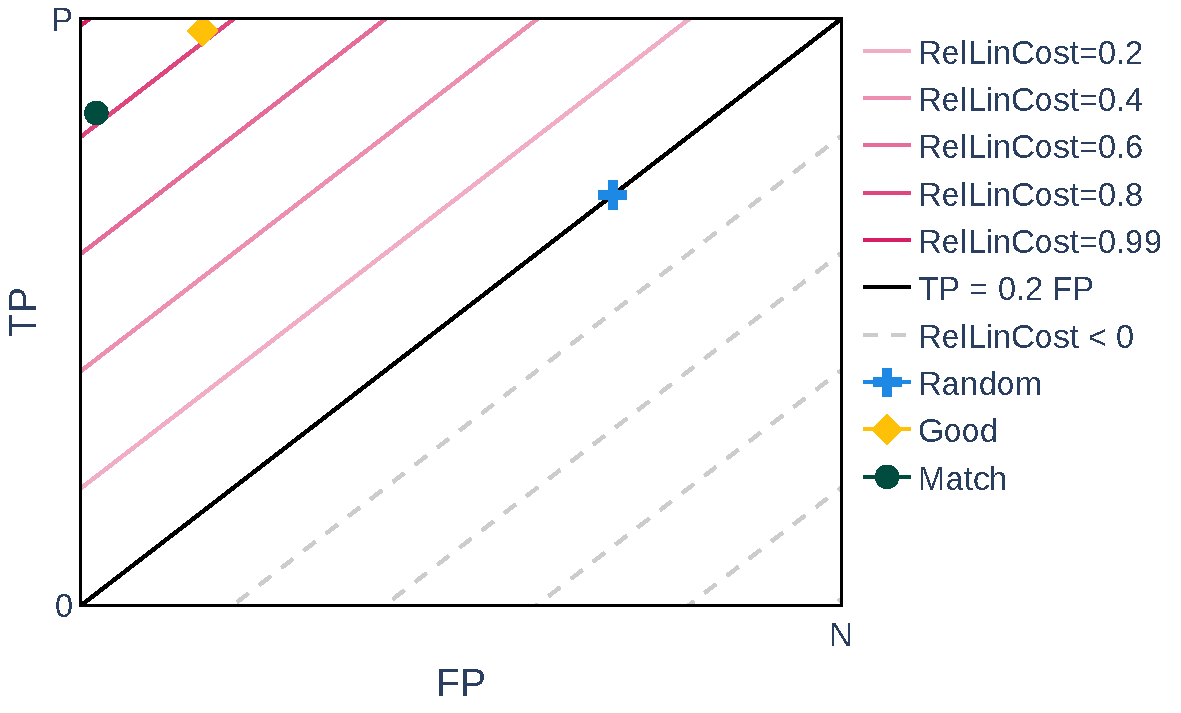
\includegraphics[width=0.7\textwidth]{Figures/MP-RelLinCost-bias}
		\caption{Isometric plot for the RelLinCost measure with a skewed class distribution.}
    \label{fig:rellincost-bias}
\end{figure}

\FloatBarrier
\subsection{Support}

Support is the most basic measure of model performance from the field of association rule learning. The definition of Support in terms of the confusion values is
$Support(\hat P, \hat N) = \frac{\hat P}{P+N}$
. An alternative definition for Support is $Support(\hat P, \hat N) = \text{P}(\hat P)$ i.e. Support is the observed probability of a true positive.
Figure \ref{fig:sup} demonstrates the isometrics of Support. These isometrics are directly perpendicular to that of MinFP, Support does not account for false positives and will thus tend towards the top-right of the coverage space when learning a rule. While Support alone is not sufficient for this work, it can be used in conjunction with another measure (commonly Confidence) to enforce a minimum number of acceptable true positives.

\begin{figure}[ht]
    \centering
    \figuretitle{Support}
    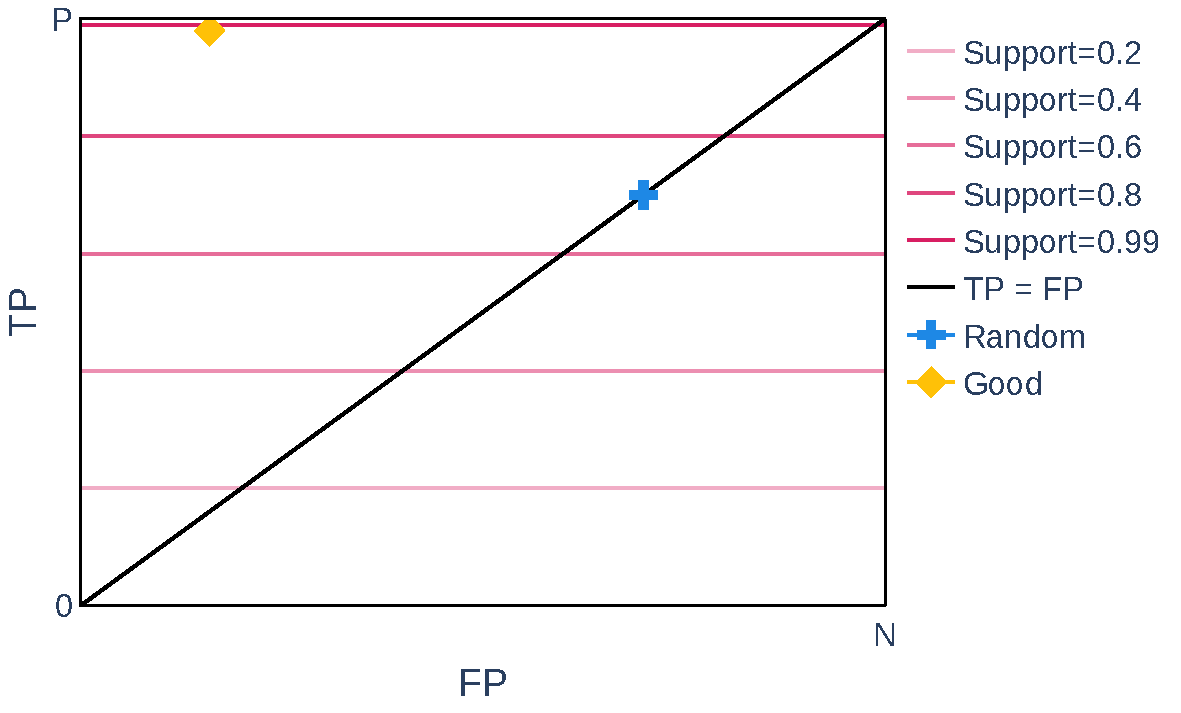
\includegraphics[width=0.7\textwidth]{Figures/MP-Support}
    \caption{Isometric plot for the Support measure.}
    \label{fig:sup}
\end{figure}

\FloatBarrier
\subsection{Confidence}

Confidence (also known as Precision) is another measure that comes out of the field of association rule learning. The definition of Confidence with respect to the confusion values is
$Confidence(\hat P, \hat N) = \frac{\hat P}{\hat P+\hat N}$
. Intuitively, Confidence is the proportion of correctly classified examples. This can also be stated as the conditional probability
\\$\text{P}(\text{Positive example}| \text{Positive classification})$. This intuition makes Confidence highly desirable when sharing results with a non-technical audience.

As can be seen in Figure \ref{fig:conf}, the Confidence measure does account for both $\hat P$ and $\hat N$. However, it only looks at the values in proportion to one another, meaning that a rule with 0 true positives can rate as high as one with $\hat P = P$. Fortunately, this can be compensated for by using the Support measure together with Confidence. Where the Support measure is used to provide a minimum threshold on the number of true positives and Confidence is used to rank models that pass that threshold. This is not always desirable, as it reduces the use of Confidence to be very similar to MinFP. However, in this work, it is preferable to minimize $\hat N$ over maximizing $\hat P$ and Confidence allows for a convenient trade-off while remaining intuitive. 

For Confidence a Match example with $\hat P$, $\hat N$, $\bar N$, and $\bar P$ of 0.3, 0.05, 0.95, 0.7 respectively are used. The Random example has a Confidence of 0.5, the Good and Match examples have a Confidence of 0.86. When the class imbalance is introduced (Figure \ref{fig:conf-bias}) the Random example Confidence becomes 0.167, the Good and Match Confidence becomes 0.55. This is better than the Accuracy example because the Good and Match examples still have the same Confidence. This means that Confidence is a suitable measure for use in the learning stage because learning algorithms (e.g. the Apriori algorithm) only rely on relative sorting of rules, which does not change in this case. However, the intuitive understanding of Confidence is no longer clear in the case of class imbalance, where a Random guess now has a Confidence of 0.167.


\begin{figure}[ht]
    \centering
    \figuretitle{Confidence}
    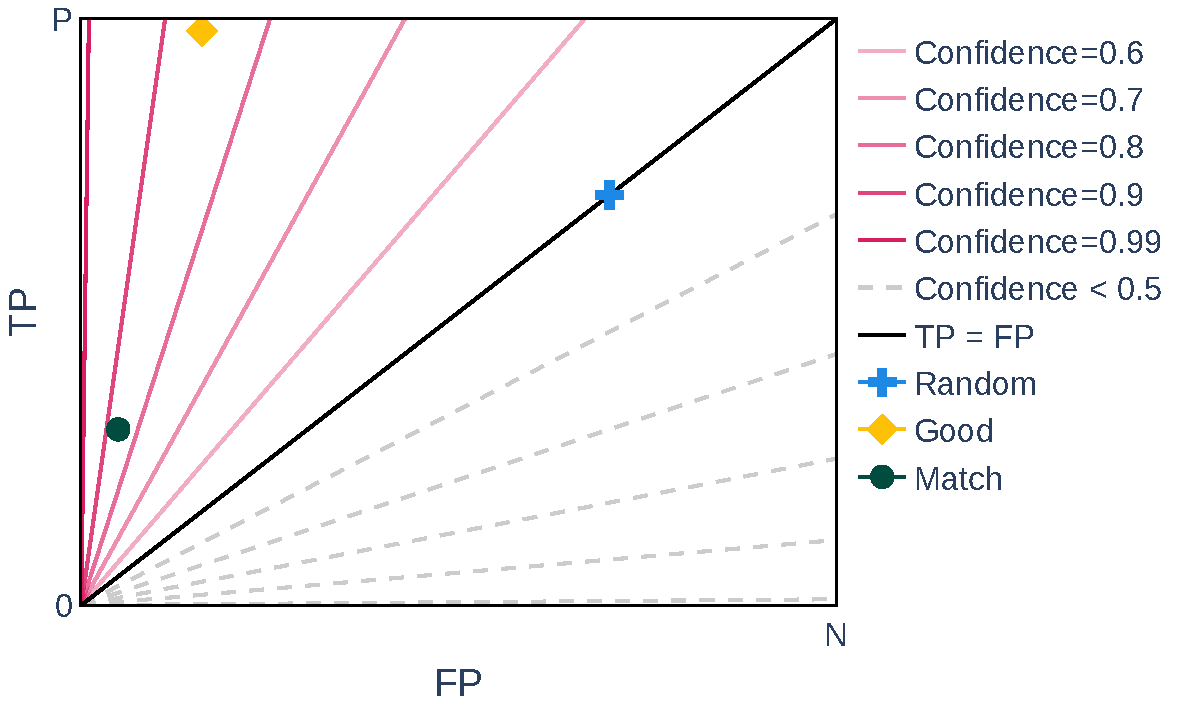
\includegraphics[width=0.7\textwidth]{Figures/MP-Confidence}
		\caption{Isometric plot for the Confidence measure.}
    \label{fig:conf}
\end{figure}
\begin{figure}[ht]
    \centering
    \figuretitle{Confidence; P = 0.2 N}
    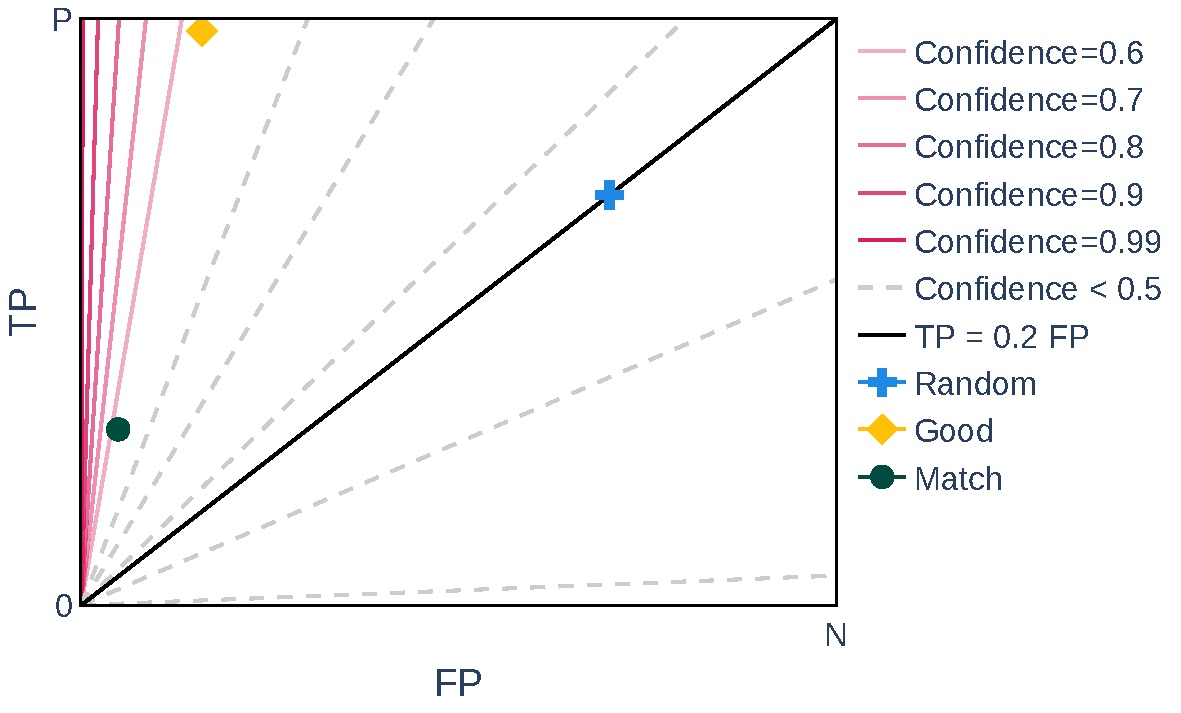
\includegraphics[width=0.7\textwidth]{Figures/MP-Confidence-bias}
		\caption{Isometric plot for the Confidence measure with a skewed class distribution.}
    \label{fig:conf-bias}
\end{figure}

\FloatBarrier
\subsection{Lift}

Lift is the final measure that comes from the field of association rule learning. The definition of Lift is
$Lift(\hat P, \hat N) = \frac{\frac{\hat P}{\hat P+\hat N}}{\frac{P}{P+ N}}$
. Intuitively, Lift is the relative performance increase (or decrease) of a classification model when compared to a random guess. In this context, a random guess is a random decision with a probability matching that of the underlying data, $\frac{P}{P+N}$ in this case. This makes judging the quality of a rule based on Lift trivially easy as and value $>1$ is by definition better than a random guess. 

Figure \ref{fig:lift} demonstrates the isometrics of Lift. As can be seen, these are identical to those of Confidence. This does not suggest that the two measures are the same, they clearly output different values, but when used to evaluate the relative performance of a machine learning model Confidence and Lift will always match.
Figure \ref{fig:lift-bias} shows the same figure under a new class distribution ($P = 0.2 N$). 
Here the Match example is the same as used with Confidence. Lift differs from Confidence because it is normalized by the underlying class distribution (similar to RelLinCost). This means that when class imbalance is introduced the values of Lift change, but the Lift value corresponding to a random guess (1) and the relative values between the Good and Match classifier do not change. This means that users do not lose the fundamental intuition that Lift $> 1$ is good, and the training system can still rely on the order of classifiers based on Lift.

Lift can also benefit from the use of Support described above. This gives Lift all the same benefits as Confidence in the context of model training, but benefits from a consistent, intuitive interpretation for any class distribution.

\begin{figure}[ht]
    \centering
    \figuretitle{Lift}
    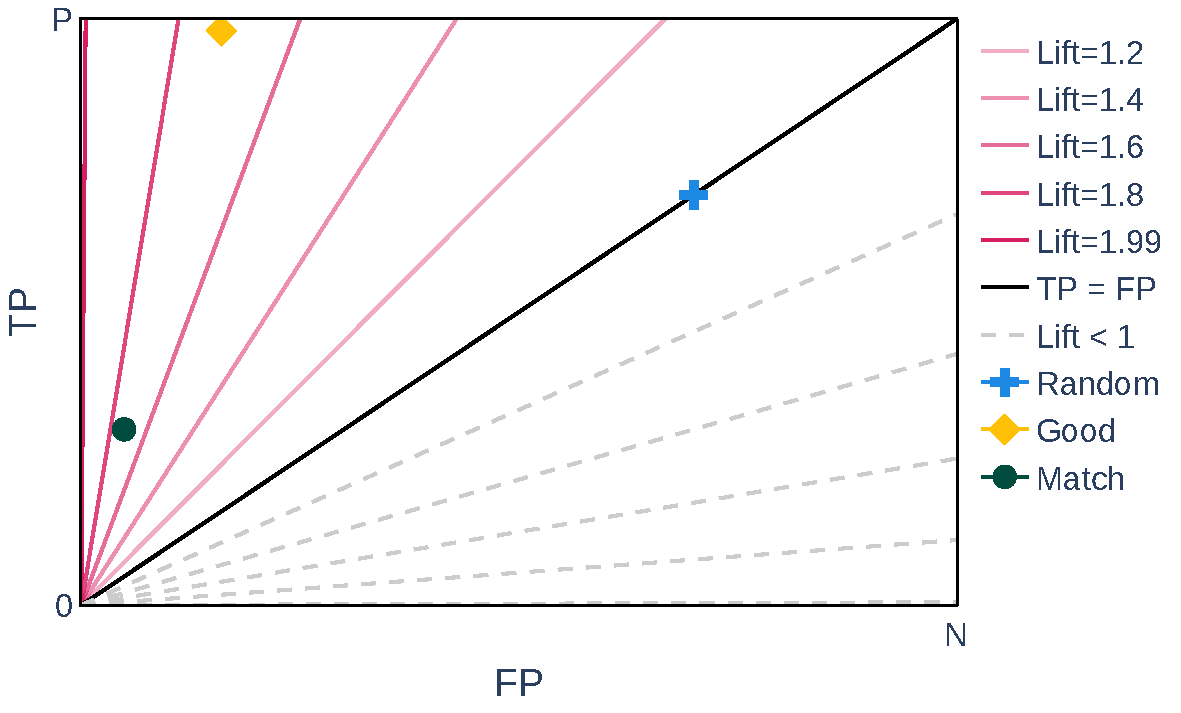
\includegraphics[width=0.7\textwidth]{Figures/MP-Lift}
		\caption{Isometric plot for the Lift measure.}
    \label{fig:lift}
\end{figure}
\begin{figure}[ht]
    \centering
    \figuretitle{Lift; P = 0.2 N}
    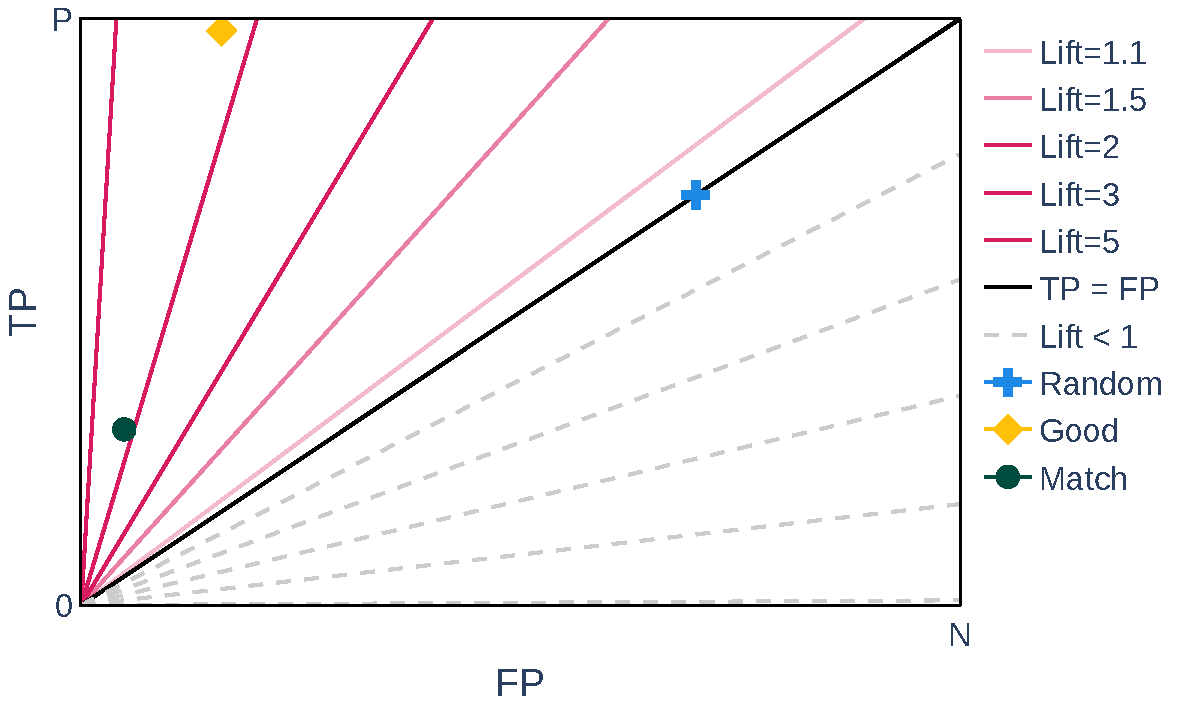
\includegraphics[width=0.7\textwidth]{Figures/MP-Lift-bias}
		\caption{Isometric plot for the Lift measure with a skewed class distribution.}
    \label{fig:lift-bias}
\end{figure}


\FloatBarrier
% \subsection{Decision}
% As transparency is a key focus of this work, it is important that the measure used for model training is the same as the measure presented to users. This prevents inconsistencies between the generated order of rules, and the order as seen by users. 

% Only RelLinCost and Lift have been identified as suitable for use in this work. Both perform well with varying class distributions and both present an intuitive understanding. For RelLinCost any values from 0-1 are improvements where 1 is the best and 0 is no improvement. For Lift any value above 1 is an improvement, the larger the better.
% Lift was selected for model training and presentation. The intuitive interpretation of Lift as "X times better than a random guess" is beneficial to users of the system who might not grasp RelLinCost and it fits with the training system introduced in chapter \ref{chap:algo}. 


\section{Conclusion}

The Accuracy, RelLinCost, Support, Confidence, and Lift measures were all discussed. It was found that Accuracy and Confidence lose their intuitive understanding when used with data sets that have a large degree of class imbalance. RelLinCost, Support, and Lift maintain the same understanding despite the change in underlying distribution. Support is lacking however in presenting the full picture of classification performance as it does not consider False Positives. RelLinCost and Lift are both suitable for use in this work, based on the above analysis. However, Lift will be the measure used in this work as it is already used by the Apriori algorithm and has a more consistent and intuitive representation than any of the other measures presented here.

